\documentclass{article} % For LaTeX2e
\usepackage{nips12submit_e,times}
\usepackage{amsmath,bbold}
\usepackage{graphicx}
\usepackage{pbox}
%\documentstyle[nips12submit_09,times,art10]{article} % For LaTeX 2.09
\newcommand{\tab}{\hspace*{2em}}

\title{Citation Recovery with Weighted Citation Network Links and Contextual Semantic Information}


\author{
Jonathan C. Barker\tab Kartik Goyal\tab Zhengzhong Liu \\
Language Technologies Institute \\
Carnegie Mellon University \\
Pittsburgh, PA 15213 \\
\texttt{\{jcbarker, kartikgo, liu\}@cs.cmu.edu} \\
}

% The \author macro works with any number of authors. There are two commands
% used to separate the names and addresses of multiple authors: \And and \AND.
%
% Using \And between authors leaves it to \LaTeX{} to determine where to break
% the lines. Using \AND forces a linebreak at that point. So, if \LaTeX{}
% puts 3 of 4 authors names on the first line, and the last on the second
% line, try using \AND instead of \And before the third author name.

\newcommand{\fix}{\marginpar{FIX}}
\newcommand{\new}{\marginpar{NEW}}

%\nipsfinalcopy % Uncomment for camera-ready version

\begin{document}


\maketitle

\begin{abstract}
	In this work, we address the problem of missing citation prediction. Current approaches to this problem include making predictions with the citation network structure and identifying them through semantic similarity. In this work, we attempt to incorporate both of these sources of information to help make better predictions. We noted the phenomenon that not all cited papers are equally important to the citing paper. Thus we adopt a supervised random walk method to learn the appropriate weights on these links using textual semantic information and cross-document topic models. We evaluate our weighted network by predicting missing citations for a paper, given the paper's current citations.
\end{abstract}

\section{Introduction}
Identifying relevant literature from electronic collections is becoming more difficult due to their rapid growth. This makes it very challenging for researchers to conduct efficient literature review. Automation of the citation prediction task then becomes necessary. Citation networks with citation links can provide us binary information about whether a link exists between the citing and the cited papers, but fail to encode information about the relative importance and relevance of each cited paper. As a result, it is difficult to draw profound conclusions from these networks about the relationships between different network nodes. We address this problem by assigning weights to network links according to their importance and relevance to the cited paper in order to mine deep information. Tasks like automatic paper recommendation and missing citation prediction can then become much more accurate. Authors can use missing citation prediction to detect any papers they might not have cited in their initial draft, while journal reviewers can be aided in detecting any relevant works which are not cited by the submitted papers.\\
	In practice, random walks techniques \cite{Backstrom:2011:SRW:1935826.1935914,Sarkar2009,Tong2006} have been employed to find node relevance in networks. These techniques generally work with a uniformly weighted network and utilize the graph structure. Our belief is that these techniques can be used more effectively if the network graph were to contain weighted links. The weights on the links could encode rich semantic information such as semantic correlation, citing patterns, shared authors and temporal proximity.\\
The major challenge in this approach is figuring out how various sources of information can be combined with the network structure. In doing so we must determine the relative importance of these sources/features with respect to the relationship score of two papers. When we have finally synthesized this information to create our weighted network we aim to show that we can use it to produce more meaningful results for tasks such as missing citation prediction and recovery.
\section{Related Work}
There are also many unsupervised methods for link prediction.  These methods mainly focus on leveraging the network structure. Liben-Nowell and Kleinnberg \cite{Liben-Nowell2007} experimented on several measures of node proximity with a co-authorship network and concluded that Adamic/Adar method gives the best performance. Kashima et.al \cite{Kashima2009} proposed a semi-supervised method using link propagation for prediction.\\
There are a few works using relational learning methods to approach this problem \cite{Taskar2003,Popescul2003}. Backstorm and Leskovec \cite{Backstrom:2011:SRW:1935826.1935914} perform supervised random walks on networks to learn the weights on the links between community members. The weighted network is used to predict future links between the members of the social network. The weights are learned by minimizing an error function on the probability of predicting incorrect and correct future links. Lao and Cohen \cite{Lao2010} use a path-constrained random walk to do this. Yu et.al \cite{Yu2012} use a topic model to restrict the search space and learn the similarity using meta-path features. These methods focus on sophisticate path formation but do not consider local deep semantic information. \\
Nallapati et al. \cite{nallapati2008joint} use topic models created with Latent Dirichlet Allocation(LDA) \cite{blei2003latent} to predict the existence of a citation link. Apart from generating words, they also generate the reference links from the topic model, thus creating a topical dependency between cited and citing papers. LDA can be also used for determining semantic correlations between two documents. Celikyilmaz et.al \cite{Celikyilmaz:2010:LBS:1867767.1867768} studied LDA-based similarity measures on the Question Answering systems. These similarity measures used both topic proportions and importance of similar words for estimating similarity.\\
\section{Method}
\textbf{Intuition:} Citation link prediction is a complicated problem which relates to many factors besides from the citation network itself, such as co-authorship, the venue or the time of the paper, an the rich textual features in the paper. Intuitively, a better algorithm should be able to combine information from different sources. A natural way of doing this is to attach feature onto the network links, various methods have been proposed, such as \cite{Liben-Nowell2007}. However it is difficult to determine which feature should be emphasized. Hence this project embraces a supervised random walk method that translate pairwise paper features into network weights, which can be interpreted as the importance of each citation in a particular paper.  On the other hand, we also realize that a normal random walk with restart (RWR) algorithm will not fit into our problem. Traditional RWR algorithm emphasize on the network similarity which prefers locally proximity nodes to the source node. However, in a citation network, authors do not only follow the citation links, sometimes they also need to cite other related papers given their research topic. Inspired by this, we also slightly modified the normal RWR algorithm by introducing topical preference walk. Common topical models like LDA \cite{blei2003latent} can be utilized.

\textbf{Learning problem:} A major challenge of this work is how to learn the relevant weights of features, we aim to learn a function that can properly assign weights based on the dataset. Here we adopt a method similar to \cite{Backstrom:2011:SRW:1935826.1935914} which optimizes a function that can assign higher random walk probability to real missing nodes versus other nodes. We believe that since this method deals with gauging the importance of a cited paper to the citing paper using both the network structure information and the semantically enriched feaures, it has the potential to outperform several approaches which either use only one of the network information and the semantic information or are focussed on just 0/1 weights between the edges instead of weighting the edges in the graph. Consider we are given a uni-directed graph $G(V,E)$(citation links only come from one paper to another paper.), a node $s$ representing the paper we are interested in. Node $s$ links to several nodes in the network. The task is to identify the other potentially connectable links $D={d_1,...,d_m}$ and avoid linking to the $L={l_1,...,l_n}$ where there should not be a link. For each edge $e_{uv}\in E$ we denote the set of pairwise features that associated with node $(u,v)$ as $\psi_{uv}$. By creating multiple pairs of $d$ and $l$, our objective is to maximize the possibility $p_d$ of recovering nodes in $D$ and minimize the possibility $p_l$ of linking to nodes in $L$. \\
	Here we use a random walk method to calculate these possibilities. In order to direct the random walk to our objective using the features, we assign each edge $e \in E$ a weight using a parameterized function $f_w(\psi)$ which combine the feature $\psi$ with the parameters $w$. So the $w$ is exactly the parameter vector that we are going to learn. Similar to \cite{Backstrom:2011:SRW:1935826.1935914}, our target is to minimize the function:
\begin{equation}
F(w)=L(w) + h(p_l - p_d)
\end{equation} 
with respect to $w$ with certain regularization function $L$ on $w$ and the loss function $h$. By taking the partial derivative of $F(w)$ we have:
\begin{equation}
\frac{\partial F(w)}{\partial w} = \frac{\partial L(w)}{\partial w} + \sum_{l,d} \frac{\partial(p_l-p_d)}{\partial w}
\end{equation}
%\intertext{By replacing $\sigma_{ld}$ with $p_l-p_d$ we have:}
\begin{equation}
\frac{\partial F(w)}{\partial w} = \frac{\partial L(w)}{\partial w} + \sum_{l,d} \frac{\partial h(\sigma_{ld})}{\partial \sigma_{ld}}(\frac{\partial(p_l)}{\partial w} - \frac{\partial(p_d)}{\partial w}  )
\end{equation}
	The relation between the possibility of linking to node $p_u$ can be related with $w$ using the transition matrix $Q$. The basic transition matrix $Q^{(0)}$ is given by:
\[
  Q_{uv} = \left\{ 
  \begin{array}{l l}
    \frac{f_w(\psi_{uv})}{\sum_t f_w(\psi_{ut})} & \quad (u,v)\in E\\
    0 & \quad \text{otherwise}\\
  \end{array} \right.
\]
	In our problem we are interested a more general $Q$ which consider the preference vector, which is given by:
\begin{equation}
Q = (1 - \alpha) Q^{(0)} + \alpha \textbf{1}(u \in P)
\end{equation}
where $P$ is the preference vector. \\
The random walk score is given by the stationary vector $p$ where:
\begin{equation}
\label{eq:eigen}
p^T = p^TQ
\end{equation} 
	Eq. \ref{eq:eigen} and the transition matrix $Q$ give us the connection between $w$ and $p$. Then we can use the gradient descent method to optimize $F(w)$. Detailed derivation can be found in \cite{Backstrom:2011:SRW:1935826.1935914}.  

	\textbf{Feature selection:} Since, we are trying to estimate the importance of a paper to the citing paper, we decided to work with features which represent the edge strengths between two papers. In choosing these feature, we consider how normal judgments should be made on citing papers. Due to the noise of our data, we still have some features could not be accurately defined (like the position of a citation in a paper), for these we use approximate measurements. Pairwise features  between a cited paper and a citing paper can be gathered from citation patterns, semantic correlation and the network metadata:
\begin{enumerate}
  \item Number of citances for the cited paper. ("citance" refers to a citing sentence in a paper)- Intuitively, if a paper is cited many times by the citing paper, then there must be a high correlation between the two papers.
  \item Co-citance score. This is defined as the number of times another paper is cited in the same citance as the target cited paper.- This feature represents the similarities between the cited papers. If multiple papers are cited in one citance, they are likely to be similar to each other and might be of equal importance to the citing paper.
  \item The number of common papers which both citing and cited papers cite.- We believe this to be an important feature because the number of common citations among the cited and the citing paper, represent the similarity between two papers.
  \item Topical similarity between the citing and cited paper, calculated using topic proportions from Latent Dirichlet Allocation(LDA). - This feature represents the semantic content based similarity.
  \item Number of common authors.- We believe this to be an important feature because same authors are likely to work together on similar topics.
  \item The difference between time of publication, measured in years. - This feature represents the temporal importance of a cited paper to the citing paper.
  \item Number of citances with the cited paper in the first third section of the paper.
  \item Number of citances with the cited paper in the middle third section of the paper.
  \item Number of citances with the cited paper in the final third  section of the paper.
\end{enumerate}
Features 7, 8, 9 are location based features, which represent importance of the cited papers on the basis of their appearances in the citances in different sections of the paper. Features 3, 5 and 6 are meta-data related to the citation network. To determine 1 and 2 we used regular expressions to extract citances and match them with the cited papers. Mallet toolkit \cite{mallet} was used for running LDA, which uses gibbs sampling for parameter inference, on the raw text of all the papers. The topic proportion vectors were created and were used to calculate cosine similarity between documents.

\textbf{Topical group exploration:} In order to simulate human's preference in choosing papers to cite, we introduce an additional preference vector into the traditional random walk. The hypothesis is simply that authors would prefer to cite papers with similar topics. This can also be viewed as a way of borrowing information or topics from the other paper. To implement this, we get a simple LDA based similarity score for all the target papers, then a normalized score vector $\textbf{T}$ is used together with the source node to create the preference vector $P$. The preference vector is given by:
\begin{equation}
P =\beta \textbf{1}(u=s) + (1-\beta)\textbf{T}
\end{equation}
\section{Experiment} 
\subsection{Experiment setup}
We are currently conducting the experiments on the ACL Anthology Network (AAN) \cite{Radev&al.09,Radev&al.09a} which contains the citation network of ACL paper collections and the relevant metadata from year 1965 to 2011 with over 15,000 papers. To simplify the experiment setting, we make a approximate assumption that papers will cite papers in the past years. After that, we choose training and testing data by year. Originally, we choose to use papers from year 2010 data as the training set with papers before 2010 as the candidate set and papers from year 2011 data (about 760 papers) are used as the testing set and all other papers are treated as the candidate set (about 14,600 papers). However, this will create a huge matrix which is difficult to be evaluated in our algorithm. We use much smaller training sets to perform training due to time and resource constraints. As a side note, there is a sparsity problem of the citation network given that a paper does not contains many citations within ACL conferences itself. Currently we cannot overcome this issue and simply ignore the papers from other venues.\\
  To generate the $D$ (target citing) and $L$ (not citing) set, we randomly remove links from each testing paper with 25\% possibility. The removed links will be treated as the $D$ set and all other links will non-existing links can be treated as $L$ set candidates. However, it is not clear that which ones of the non-existing links should be used as the $L$ set. There can be some papers that are very similar to the citing paper but not got cited for various reasons.\\
As pointed out by \cite{nallapati2008joint}, normal metrics such as precision and recall are not suitable for this task because we do not expect a paper to cite all relevant papers. We adopt their metric RKL (short for RanK Last), which represent the rank of the last citation we recovered. On the other hand, we are also interested when we can get the first correct prediction, so we introduce another metric RKF (short for Rank First).\\

\subsection{Experiment results and discussion:} 
In the experiments, there are several decisions that we are going to evaluate. (A) Selection of preference vector; (B) Selection of restart possibility $\alpha$; (C) Selection of $\beta$ (used for calculating preference vector); (D) Experiments on feature selection; (E) Distribution of RKF and RKL to realize the effect of random outliers on average RKF and RKL. The experiments regarding to the learning method will be discussed in Section \ref{sec:learning}.\\
\\
\textbf{(A) Basic model and preference vector}.\\ 
The purpose of our method is to mine possible papers for citation using weights to direct the random walk. In the basic model, we perform some experiments using uniform weights to investigate the utility of combining semantic information with graph structure. The selection of the preference vector also plays an important role. Random Walk with Restart (RWR) has proved to be useful in looking for similar nodes in neighbors  \cite{Backstrom:2011:SRW:1935826.1935914,Tong2006}. However, in a paper the author would not only cite papers that have links with each other. We make the hypothesis that the author of a paper should be more likely to cite papers in multiple topic groups corresponding to the topics discussed by the paper. Thus it makes sense to set the preference vector based on the topical similarity with the target document. To verify the hypothesis, we conduct some simple experiments. We consider different the combination of random walk and LDA model using Cosine similarity over topic distribution similarity. In addition, we consider different handling over the dangling nodes. In "Strongly preferenced" mode, we patch all dangling nodes, adding transitions following our preference vector. In "Weakly preferenced" mode, we patch them with a uniform transition towards all other nodes. We use the WebGraph\cite{Boldi2004} package to do the experiments. Different combinations give us 5 different experiments.\\
The preference vector $P$ is stochastic, we assign to the target node $s$ a preference $\beta (0< \beta <1)$. Then we assign the rest $1-\beta$ weights to all the other nodes in proportion to their similarity with $s$. In this experiment, $\beta$ is set as 0.2 and $\alpha$ is 0.6 .\\
The different experimental results are shown in table \ref{results-table}. The general trend shows that "weakly preferenced" performs better than "strongly preferenced". This could be related to that jumping from dangling nodes to our preferred node does not help exploring the network. On the other hand, we can see that simple LDA similarity outperforms the basic RWR, this is consistent with our hypothesis that author would prefer to cite papers in multiple topical groups. However, the combination of LDA and RWR gives the best performance, which is consistent with our hypothesis. It is also a positive sign that our method of combining semantic and network information is effective. Overall, combining RWR with LDA shows a more robust result.\\
In additional to the average score, it is also interesting to see the distribution of the points in order to understand the practical value of the method. In Fig. \ref{fig:RKF} and \ref{fig:RKL} we show the distributions of RKF and RKL with $\alpha=0.6$ and $\beta=0.1$ (considerably the best performance). We plot the histogram of the rank distribution of our more than 700 test instances. We see in Fig. \ref{fig:RKF}, the distribution of RKF, the there is a large peak for the lower values of RKF and a sharp drop in frequency for higher values. This tells us that the mean of the distribution is closer to the most likely RKF but we do observe some outliers. The lower standard deviation gives us more confident that the RKF performs quite consistently, which means our method can quickly identify the first paper to cite in a rather robust manner.\\
In Fig. \ref{fig:RKL}, from the distribution of RKL, we see a more gradual drop in frequency as RKL increases. There are a few high values in several regions. Clearly, RKL is more deviated from the mean. This is expected because sometime some citations are only barely mentioned and very loosely connected with the citing paper. Also, when we hides some links in the testing set (sometimes we get zero links left but we filter out these instances), there is a probability that we remove all the links from the source paper to a particular region in the graph, this will make discovering the citation very hard (which can be reflected in the more frequent long tail in the distribution). From a practical point of view, it is unlikely that one paper will totally ignore a whole field of related citations, thus our algorithm are expected to perform at a level closer to the mean in practice.\\
\begin{table}[t]
\caption{Experiment on Basic Model and Preference Vector}
\label{results-table}
\begin{center}
\begin{tabular}{llllllll}
\multicolumn{1}{c}{\bf Method}  &\multicolumn{1}{c}{\bf $\bar x$ RKF} &\multicolumn{1}{c}{\bf $\bar x$ RKL} &\multicolumn{1}{c}{\bf $SD$ RKF} &\multicolumn{1}{c}{\bf $SD$ RKL} &\multicolumn{1}{c}{\bf Med. RKF} &\multicolumn{1}{c}{\bf Med. RKL}
\\ \hline \\
 {RWR (weakly  preference)} & 1084.33 & 4523.92 & 2256.77 & 4494.55 & 28 & 4822\\
 {RWR (strongly  preference)}& 1692.63 & 6123.96 & 2298.70 & 4545.55 & 28 & 5514\\
{LDA similarity}  & 392.57 & 2460.04 & 699.78 & 4211.32 & 46 & 863\\
{RWR with LDA}  (weakly) &\textbf{151.04} &\textbf{809.23} & \textbf{219.14} & \textbf{1205.56} & \textbf{41} & \textbf{375}\\
{RWR with LDA}  (strongly) & 162.83 & 850.92 & 1098.41 & 4227.90 & 47 & 1032\\
\end{tabular}
\end{center}
\end{table}

\begin{figure}[ht]
\begin{minipage}[b]{0.6\linewidth}
\centering
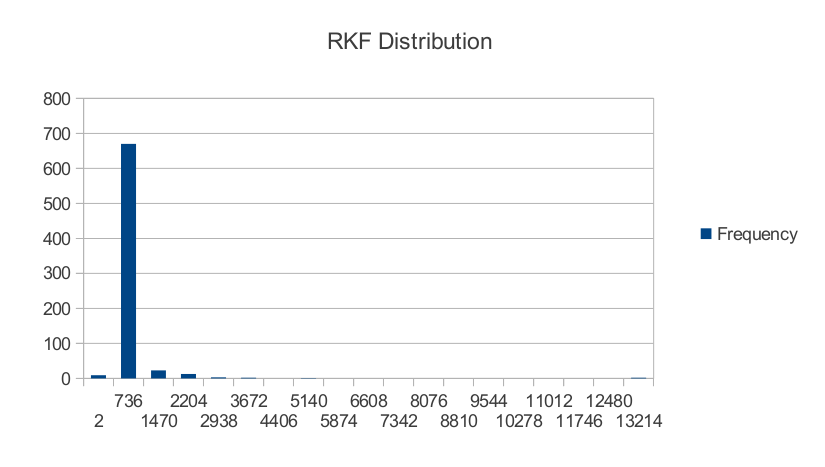
\includegraphics[width=\textwidth]{rkf.png}
\caption{Distribution of RKF for $\alpha=0.6$, $\beta=0.2$}
\label{fig:RKF}
\end{minipage}
\hspace{0.2cm}
\begin{minipage}[b]{0.6\linewidth}
\centering
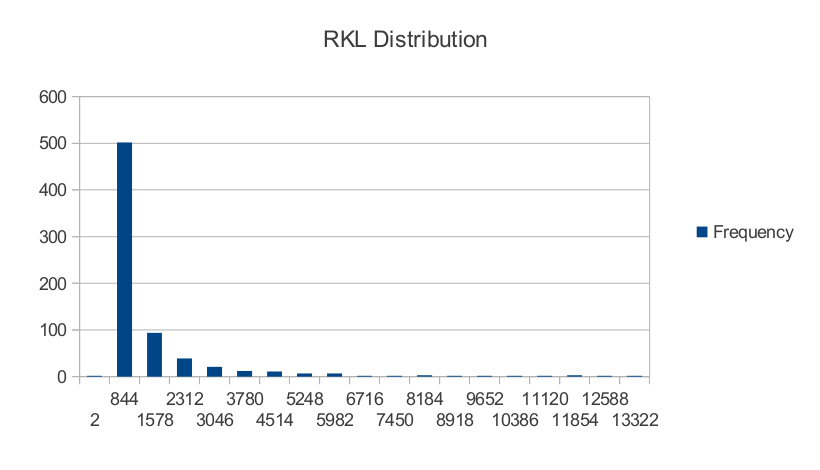
\includegraphics[width=\textwidth]{rkl.png}
\caption{Distribution of RKL for $\alpha=0.6$, $\beta=0.2$}
\label{fig:RKL}
\end{minipage}
\end{figure}

\textbf{(B) Selection of restart probability.}\\
In this experiment we test the effect of different $\alpha$ values on the basic random walk method. In Fig. \ref{fig:evalAlpha} we can see that the performances with different $\alpha$ are similar except when close to the two ends (0 or 1). We observe that the RKF and RKL values do not vary too much between $\alpha$ values 0.2 and 0.8. This shows that the performance does not change significantly with the change of $\alpha$. One explanation is that the RWR will generally assign higher score to closer nodes the more distant nodes, even when the random walk distance is high (when $\alpha$ is small). It could also be related to the sparsity of the network, which results in very concentrated local networks.\\ 
\begin{figure}[htb]
\centering
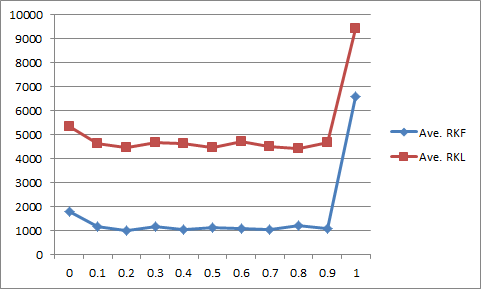
\includegraphics[width=0.5\textwidth]{evalAlpha}
\caption{Behavior of different alpha value in basic random walk}
\label{fig:evalAlpha}
\end{figure}
\\
\textbf{(C) Selection of $\beta$ (used for calculating preference vector)}\\
In Fig. \ref{fig:evalBeta} we see the results of using different $\beta$ values for the weakly preference random walk method. The general trend of RKF and RKL is to increase slightly as $\beta$ increases (so that more weights will be assign to the source node), RKL increasing more rapidly. As discussed before, $1-\beta$ represents the strength of the random walk's dependence of the preference vector. These results shows that the random walk method greatly benefits from a topical similarity-based preference vector using LDA, that our hypothesis of exploring the whole network holds here.\\
\begin{figure}[htb]
\centering
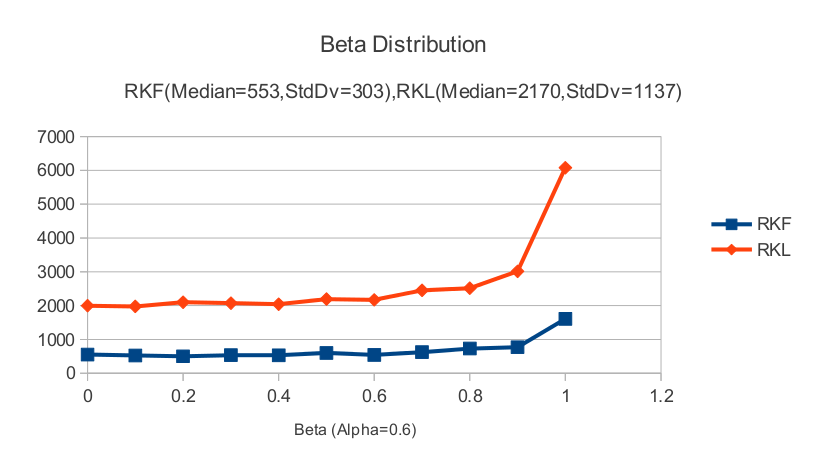
\includegraphics[width=0.8\textwidth]{beta.png}
\caption{Behavior of different beta values in weakly preferred random walk}
\label{fig:evalBeta}
\end{figure}
\\
\textbf{(D) Experiments on feature selection}\\
Before training, we decided to explore the relative importance of our features. In this experiment for each feature we tried setting the weight to 1.0 and all others to 0.0. Then we ran weakly preferenced random walk using the LDA-based preference vector and these feature weights. In the end, all evaluations yielded similar results. The average RKF was approximately 190 and the average RKL was approximately 900. This tells us that none of our features seem to be particularly more important than the others, so they must be trained together to yield better results. The disparity between the average RKF and RKL values for this experiment and the experiment using uniform feature weights shows that biasing the walk for a particular feature heavily decreasing performance. We also impose doubts on whether the method can successfully leant the model giving the sparsity network, the problem is addressed in subsection \ref{sec:learning}\\
%
\subsection{Experiments on learning algorithm}
\label{sec:learning}
The training algorithm is tested on a smaller data set using year 1990's paper as training source and the years before it as candidates pool. There are about 73 training sources. However, the training algorithm does not shows a satisfying result. When choosing the initial parameters $W$ as zero vector, the training derivative goes to very small values and stops immediately. However, currently a uniform stochastic $W$ can converge to some points but random initialization cannot easily converge. We realize that the problem is not convex in general, so choosing different starting points can have effects on the learning. \\
The experiment result is shown in \textbf{Table. \ref{trained-test}}, the result is slightly worse than the best RWR + LDA method.\\
\begin{table}[t]
\caption{Test results using trained weighted RWR with LDA (weakly)}
\label{trained-test}
\begin{center}
\begin{tabular}{lll}
\bf Measure & \bf RKF & \bf RKL\\
\hline \\
Mean & 169.13 & 909.62\\
Median & 43 & 404\\
Standard Deviation & 897.59 & 2117.16\\
\end{tabular}
\end{center}
\end{table}
Besides from the fact that we only have the resource to run the experiment in a small dataset. There are several other possible causes for this phenomenon, one is that the network is too sparse that only a few links exists for one paper, it is very normal that for our training examples, there are only 1 or 2 links left for one particular paper. However, we generalize about 50 instances from each training source by arbitrarily choosing about 50 links from the $L$ (non-destination set). This could perform poorly in training because no matter what weights get assigned it is still necessary to walk to the other nodes from one existing, and it is hard to rank only one positive instances higher than many negative instances.\\
In future experiments, we propose to use real hand labelled data to generate the set of $L$ instead of randomly choosing (this is consider harmful because not cited papers doesn't mean it cannot be cited). Also, the experiment could be more successful if applying on a more self-contained and less-sparse network so that there will be fewer links that cannot be traced. Such network could be a very self-closing research field, and it would be better to use Journal collections because those articles are likely to contain more rich citations.
As discussed above, these several factors result in weighted links performing slightly worse than unweighted links using RWR with weakly preferenced LDA.
\section{Conclusion and future works}
We have observed from our results that graph structure information along with semantic correlation improves the detection of missing links.  It is shown that a simple method that combining the topical similarities with random walk provide a amazingly good result. We hypothesize this phenomena as simulating the behavior of human adding citations: people generally add citations in order to support different small aspects of the work. Thus it is useful to explore more topical groups in the network. Using a topical preferred random walk also helps us to escape the local circle created by the sparsity of the data.\\
From the experiments we observe that the behavior of our method is very much related to the network structure, but the restart related parameters $\alpha$ and $\beta$ have only limited effect on our results. This phenomena was also discovered by Backstrom et. al. \cite{Backstrom:2011:SRW:1935826.1935914}. We are using very different types of network. They used the Facebook network which has very rich links and is quite dense (while our network is largely sparse and dispersed.) This could imply a common property of RWR on such problems, though more experiments need to be conduct to confirm the result. \\
Due to various reasons, a learned RWR does not outperform the original method. We suspect this is largely related to the sparsity of the network, as there are only very limited links branch out from a paper, it is difficult to learn a weight that will bias the random walk algorithm in the right direction. Another problem could lie in our selection of training examples, though we generate the positive example using existing links, it is not clear how to choose negative examples because we lack of ground truth that some papers are really not worth citing.\\ 
There are also some other types of information that we have not fully utilize, such as co-author networks. In fact, it is proven in literature that a heterogeneous network can provide more information and thus give better prediction \cite{Lao2010,Yu2012}. Also, a heterogeneous network would be less sparse and can be attached with more information on it which largely prevent the data sparseness problem.\\
As an alternative approach to the problem of citation recovery we could simply use 1/0 weights which represent the existence or non-existance of edges in the network to perform binary classification. However, this approach would remove the information about how important cited papers are to citing papers.

\newpage
\bibliographystyle{plain}
\bibliography{midrep}
\nocite{*}

\end{document}
